\newpage
% \section{Interface Web (Espace Enseigne \& Admin)}
% \subsection{Espace Commerçant}
% \begin{itemize}
%     \item \textbf{Gestion des locaux :} Ajout de points de vente avec adresses distinctes (géocodage GPS).
%     \item \textbf{Tableau de bord :} Statistiques de livraisons, suivi en temps réel sur carte.
%     \item \textbf{Abonnement :} Sélection du plan tarifaire (Bronze, Or, etc.) via Stripe Billing.
%     \item \textbf{API Keys :} Génération de clés uniques par local pour la liaison avec le plugin.
% \end{itemize}

% \subsection{Espace Administrateur}
% Interface de gestion interne pour la validation des documents légaux (Kbis, ID) et la vue globale des opérations.



% N'oublie pas d'ajouter ces lignes dans le préambule de ton main.tex si ce n'est pas déjà fait :
% \usepackage{tikz}
% \usetikzlibrary{arrows.meta, positioning, calc}
% \usepackage{tabularx}
% \usepackage{booktabs}

\section{Conception de l'Interface Web et Logique Applicative}
\label{sec:interface_web}

L'interface Web constitue le poste de contrôle principal pour les commerçants et l'outil de régulation pour les administrateurs. Cette section détaille les choix technologiques, la modélisation des états et les directives de conception pour garantir une plateforme réactive et maintenable.

\subsection{Choix Technologiques (La Stack)}

Il est impératif d'utiliser une stack moderne qui favorise la réactivité (temps réel) et la maintenabilité du code.

\begin{table}[ht!]
    \centering
    \renewcommand{\arraystretch}{1.3}
    \begin{tabularx}{\textwidth}{@{} l l X @{}}
        \toprule
        \textbf{Composant} & \textbf{Technologie} & \textbf{Justification} \\
        \midrule
        \textbf{Framework} & Next.js 14+ (App Router) & Rendu hybride (SSR/Client), routing robuste et optimisation SEO du site vitrine. \\
        \textbf{Langage} & TypeScript & Typage strict pour sécuriser la manipulation des objets complexes (Commande, Utilisateur). \\
        \textbf{Styling} & Tailwind CSS + Shadcn/UI & Design système cohérent, implémentation rapide et accessibilité (normes ARIA) native. \\
        \textbf{Gestion d'état} & TanStack Query & Gestion ultra-performante du cache serveur et des synchronisations avec l'API. \\
        \textbf{Temps Réel} & WebSockets (Socket.io) & Crucial pour le suivi GPS du livreur en direct sans rafraîchissement de la page. \\
        \bottomrule
    \end{tabularx}
    \caption{Stack technologique de l'interface Web}
    \label{tab:tech_stack}
\end{table}

\subsection{Modélisation des États de l'Interface}

L'interface utilisateur est directement pilotée par l'état (statut) de la commande. Le diagramme d'états ci-dessous représente le cycle de vie d'une vue de commande côté Commerçant.

\begin{figure}[ht!]
    \centering
    \begin{tikzpicture}[
        node distance=1.5cm and 2cm,
        state/.style={draw, thick, rounded corners, fill=blue!5, minimum width=3.5cm, minimum height=1cm, align=center},
        arrow/.style={->, >=stealth, thick}
    ]

    % Noeuds
    \node[state] (draft) {Brouillon / En attente};
    \node[state, right=of draft] (searching) {Recherche Livreur};
    \node[state, below=of searching] (pickup) {Livreur en route\\(Collecte)};
    \node[state, left=of pickup] (delivery) {En cours de livraison\\(Transport)};
    \node[state, below=of delivery] (done) {Livré / Clôturé};

    % Flèches
    \draw[arrow] (draft) -- node[above, font=\scriptsize]{Validation API} (searching);
    \draw[arrow] (searching) -- node[right, font=\scriptsize]{Acceptation} (pickup);
    \draw[arrow] (pickup) -- node[above, font=\scriptsize]{Code A valide} (delivery);
    \draw[arrow] (delivery) -- node[left, font=\scriptsize]{Code B valide} (done);

    \end{tikzpicture}
    \caption{Diagramme d'états du cycle de vie d'une commande (Vue Commerçant).}
    \label{fig:state_diagram_order}
\end{figure}

\subsection{Architecture des Dashboards}

L'application Web se divise en trois grandes zones isolées et sécurisées selon le rôle de l'utilisateur :

\subsubsection{Dashboard Commerçant (La Tour de Contrôle)}
\begin{itemize}
    \item \textbf{Vue Carte :} Intégration d'une cartographie (ex: Google Maps, ...) pour géolocaliser les livreurs affectés en temps réel.
    \item \textbf{Gestion API :} Interface dédiée pour générer/révoquer des locaux ou boutiques physiques.
    \item \textbf{Validation Handshake :} Interface d'affichage bien visible du \textbf{Code A} à transmettre au livreur lors de son arrivée au local.
\end{itemize}

\subsubsection{Panel Administrateur (Le Back-Office)}
\begin{itemize}
    \item \textbf{Files d'attente KYC :} Interface de revue des pièces d'identité des livreurs avec outils de zoom, validation ou rejet avec motif.
    \item \textbf{Arbitrage et Monitoring :} Console d'intervention permettant de forcer l'annulation ou la validation d'une course bloquée en cas de litige.
\end{itemize}

\subsubsection{Interface Web Livreur (Responsive)}
\begin{itemize}
    \item Bien que l'application mobile native soit l'outil principal du livreur sur le terrain, une version Web responsive (PWA) lui permet de gérer son profil administratif, de consulter ses factures et de demander ses virements depuis un ordinateur.
\end{itemize}

\subsection{Flux de données en Temps Réel (Séquence UI)}

L'utilisation des WebSockets permet de mettre à jour l'interface sans action de l'utilisateur. Le diagramme suivant illustre la séquence de mise à jour "Push" lorsqu'un livreur accepte une course.

\begin{figure}[ht!]
    \centering
    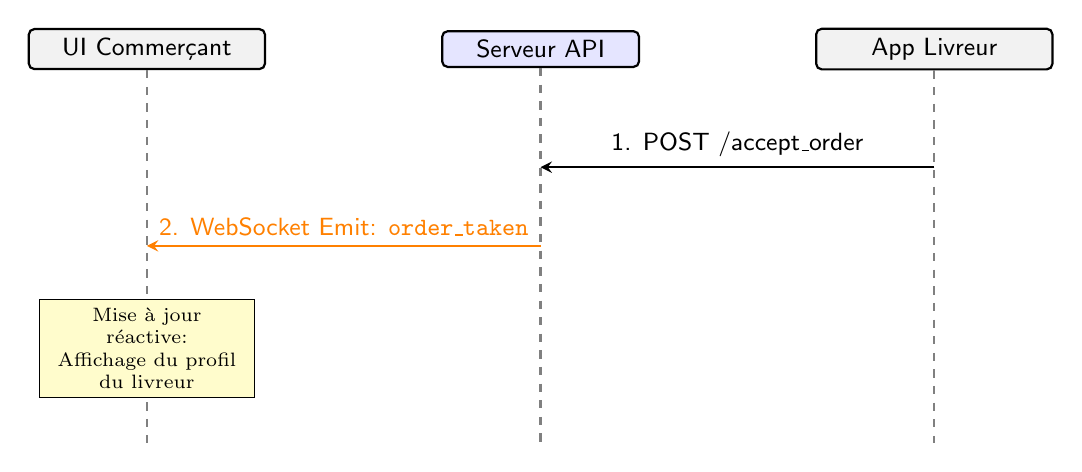
\begin{tikzpicture}[font=\sffamily\small, >=stealth]
        % Acteurs
        \node (C) at (0,0) [draw, thick, fill=gray!10, minimum width=3cm, rounded corners=2pt] {UI Commerçant};
        \node (S) at (5,0) [draw, thick, fill=blue!10, minimum width=2.5cm, rounded corners=2pt] {Serveur API};
        \node (L) at (10,0) [draw, thick, fill=gray!10, minimum width=3cm, rounded corners=2pt] {App Livreur};

        % Lignes de vie
        \draw[dashed, thick, gray] (C) -- (0,-5);
        \draw[dashed, thick, gray] (S) -- (5,-5);
        \draw[dashed, thick, gray] (L) -- (10,-5);

        % Messages
        \draw[->, thick] (10,-1.5) -- node[above]{1. POST /accept\_order} (5,-1.5);
        \draw[->, thick, color=orange] (5,-2.5) -- node[above]{2. WebSocket Emit: \texttt{order\_taken}} (0,-2.5);
        
        % Note de mise à jour UI
        \node[draw, fill=yellow!20, font=\scriptsize, align=center, text width=2.5cm] at (0,-3.8) {Mise à jour réactive:\\Affichage du profil\\du livreur};
    \end{tikzpicture}
    \caption{Séquence de mise à jour asynchrone de l'interface via WebSockets.}
    \label{fig:seq_websocket_ui}
\end{figure}



\subsection{Directives Techniques : Langages et Frameworks (Stack Front-End)}

Afin d'assurer une base de code homogène, maintenable et performante, l'équipe de développement devra maîtriser et appliquer rigoureusement la stack technologique suivante pour toute l'interface Web :

\subsubsection{Cœur de l'Application (Framework \& Langage)}
\begin{itemize}
    \item \textbf{Next.js (Framework basé sur React) :} Il s'agit du moteur principal de l'application Web. Les développeurs devront utiliser le nouveau paradigme \textit{App Router}. Il est crucial pour l'équipe de comprendre la distinction entre les \textit{Server Components} (utilisés pour le rendu rapide et le SEO des pages publiques) et les \textit{Client Components} (réservés aux dashboards interactifs nécessitant des \textit{Hooks} React comme les tableaux de bord commerçant et admin).
    \item \textbf{TypeScript (Langage) :} L'intégralité du projet front-end sera codée en TypeScript. Les développeurs ont pour directive d'utiliser un typage strict (\texttt{strict: true} dans la configuration). Ils devront définir des \textit{Interfaces} et des \textit{Types} clairs pour les entités métier (Commande, Livreur, StatutHandshake) afin d'éliminer les erreurs d'exécution liées aux données de l'API.
\end{itemize}

\subsubsection{Intégration Graphique et Composants (UI)}
\begin{itemize}
    \item \textbf{Tailwind CSS (Styling) :} Les développeurs utiliseront l'approche utilitaire de Tailwind directement dans le code JSX/TSX. Cela garantit un design 100\% responsif (mobile-first) et évite le code CSS mort.
    \item \textbf{Shadcn/UI \& Radix UI (Composants de base) :} Plutôt que de coder les éléments interactifs complexes de zéro (modales de validation de codes, menus déroulants, popovers), les développeurs utiliseront ces bibliothèques. Cela garantit un comportement natif parfait et le respect strict des normes d'accessibilité (ARIA).
\end{itemize}

\subsubsection{Gestion des Données, Formulaires et Temps Réel}
\begin{itemize}
    \item \textbf{TanStack Query / React Query (Data Fetching) :} Pour toutes les requêtes REST standards (historique, récupération de profil). React Query gérera le cache, la re-validation en arrière-plan et fournira nativement les états de chargement (\texttt{isLoading}) et d'erreur.
    \item \textbf{React Hook Form + Zod (Formulaires) :} La création de compte (Commerçant/Livreur) et la soumission du KYC nécessitent des formulaires robustes. Zod sera utilisé pour définir le schéma de validation (ex: vérifier qu'un code postal est valide) et React Hook Form gérera les saisies utilisateur sans provoquer de re-rendus inutiles de l'interface.
    \item \textbf{Socket.io-client (WebSockets) :} Pour le suivi GPS et les notifications en direct. Les développeurs devront encapsuler la logique WebSocket dans des \textit{Hooks} personnalisés (ex: \texttt{useOrderTracking()}) qui écouteront les événements du serveur et déclencheront les changements d'état locaux dans les \textit{Client Components} de React.
\end{itemize}